\documentclass[12pt,a4paper]{report}
\usepackage{amsmath,amssymb,amsthm}
\usepackage{graphicx}
\graphicspath{{./}{figs/}}
\usepackage{tikz}
\usetikzlibrary{shapes.geometric,arrows.meta,positioning,calc,decorations.pathreplacing,shadows,fit}
\usepackage{pgfplots}
\pgfplotsset{compat=1.18}
\usepackage{pgfgantt}
\usepackage{booktabs}
\usepackage{longtable}
\usepackage{array}
\usepackage{multirow}
\usepackage{setspace}
\usepackage{xcolor}
\usepackage{caption}
\usepackage[hidelinks,colorlinks=true,linkcolor=blue!50!black,citecolor=teal!60!black,urlcolor=blue!60!black]{hyperref}
\usepackage[numbers,square,sort&compress]{natbib}
\usepackage{fancyhdr}
\usepackage{titlesec}
\usepackage{tocloft}
\usepackage{geometry}
\geometry{a4paper,top=3cm,bottom=3cm,left=2.8cm,right=2.8cm}
\linespread{1.5}
\usepackage[extrafootnotefeatures]{xepersian}
\settextfont{XB Niloofar}
\setlatintextfont{Times New Roman}
\setdigitfont{Yas}

%======================= تنظیمات ظاهری =======================
\definecolor{navydeep}{RGB}{20,40,90}
\definecolor{goldacc}{RGB}{180,140,40}

\titleformat{\chapter}[display]
  {\normalfont\bfseries\Huge\color{navydeep}}
  {\filright\Large فصل \thechapter}
  {8pt}
  {\filright}
\titlespacing*{\chapter}{0pt}{-10pt}{25pt}

\pagestyle{fancy}
\fancyhf{}
\fancyhead[C]{\small پروپوزال طرح ملی زیرساخت توزیع کلید کوانتومی و رمزنگاری پساکوانتومی}
\fancyfoot[C]{\thepage}
\renewcommand{\headrulewidth}{0.4pt}

\theoremstyle{plain}
\newtheorem{theorem}{قضیه}[chapter]
\newtheorem{definition}{تعریف}[chapter]
\newtheorem{corollary}{نتیجه}[chapter]

\newcommand{\Cite}[1]{\lr{\cite{#1}}}

%======================= اطلاعات سند =======================
\title{\textbf{\Huge پروپوزال طرح ملی\\[6pt]
پیاده‌سازی زیرساخت توزیع کلید کوانتومی \lr{(QKD)}\\
و رمزنگاری پساکوانتومی \lr{(PQC)}\\[4pt]
\Large با تمرکز بر امنیت سایبری و شبکهٔ بانکی کلان‌شهر تهران}}
\author{تهیه‌شده جهت ارائه به: \\ صندوق نوآوری و شکوفایی و معاونت علمی، فناوری و اقتصاد دانش‌بنیان ریاست‌جمهوری}
\date{مرداد \lr{1405} -- آگوست \lr{2026}}

\begin{document}

\begin{titlepage}
\centering
\vspace*{1cm}
{\large \lr{Islamic Republic of Iran}}\\[0.3cm]
{\large معاونت علمی، فناوری و اقتصاد دانش‌بنیان ریاست‌جمهوری}\\[1.7cm]

\rule{\linewidth}{1pt}\\[0.6cm]
{\Huge \bfseries \color{navydeep} پروپوزال طرح ملی}\\[0.4cm]
{\huge \bfseries پیاده‌سازی زیرساخت توزیع کلید کوانتومی}\\[0.2cm]
{\Large \lr{(Quantum Key Distribution -- QKD)}}\\[0.5cm]
{\huge \bfseries و رمزنگاری پساکوانتومی}\\[0.2cm]
{\Large \lr{(Post-Quantum Cryptography -- PQC)}}\\[0.6cm]
{\large با تمرکز بر امنیت سایبری، زیرساخت‌های حیاتی و شبکهٔ بانکی کلان‌شهر تهران}\\[0.6cm]
\rule{\linewidth}{1pt}\\[2cm]

\begin{tikzpicture}
\node[draw=navydeep,thick,rounded corners,inner sep=14pt,fill=navydeep!4]{
\begin{minipage}{0.72\linewidth}
\centering
\textbf{کلیدواژه‌ها:} \lr{QKD}، رمزنگاری پساکوانتومی، \lr{BB84}، گره مورد اعتماد، امنیت بانکی، \lr{ML-KEM}، \lr{ML-DSA}، زیرساخت کلان‌شهری، تهران
\end{minipage}
};
\end{tikzpicture}

\vfill

{\large تهیه‌شده جهت ارائه به:}\\
{\large \bfseries صندوق نوآوری و شکوفایی و معاونت علمی، فناوری و اقتصاد دانش‌بنیان ریاست‌جمهوری}\\[1cm]
{\large مرداد \lr{1405} -- آگوست \lr{2026}}
\vspace{1cm}
\end{titlepage}

\pagenumbering{gobble}
\chapter*{چکیدهٔ اجرایی}
\addcontentsline{toc}{chapter}{چکیدهٔ اجرایی}

پیشرفت روزافزون رایانش کوانتومی، به‌ویژه بلوغ الگوریتم‌های تجزیهٔ اعداد صحیح نظیر الگوریتم \lr{\cite{shor1997}}، امنیت زیرساخت‌های رمزنگاری کلید عمومی کنونی -- شامل \lr{RSA}\LTRfootnote{Rivest--Shamir--Adleman} و \lr{ECC}\LTRfootnote{Elliptic Curve Cryptography} -- را که ستون فقرات تراکنش‌های بانکی، امضای دیجیتال و ارتباطات محرمانهٔ دولتی هستند، در افق یک تا دو دهه با تهدید جدی مواجه می‌کند. این تهدید تنها به آینده محدود نمی‌شود؛ حملات موسوم به «برداشت اکنون، رمزگشایی بعداً» \lr{(Harvest Now, Decrypt Later)} به این معناست که داده‌های رمزشدهٔ امروز، در صورت رهگیری و ذخیره‌سازی، می‌توانند در آینده توسط یک رایانهٔ کوانتومی رمزگشایی شوند. این پروپوزال دو راهکار مکمل و در حال بلوغ صنعتی را برای مقابله با این تهدید بررسی می‌کند: نخست، توزیع کلید کوانتومی \lr{(QKD)} که با تکیه بر قوانین بنیادین فیزیک کوانتومی -- به‌ویژه قضیهٔ عدم-شبیه‌سازی \lr{\cite{wootters1982}} -- امنیت تبادل کلید را نه بر پیچیدگی محاسباتی، بلکه بر قوانین فیزیک استوار می‌کند؛ و دوم، رمزنگاری پساکوانتومی \lr{(PQC)} که با استانداردهای تازه نهایی‌شدهٔ \lr{NIST}\LTRfootnote{National Institute of Standards and Technology (United States)} یعنی \lr{ML-KEM (FIPS 203)}، \lr{ML-DSA (FIPS 204)} و \lr{SLH-DSA (FIPS 205)} \lr{\cite{nist2024release}} امکان مهاجرت نرم‌افزاری و مقیاس‌پذیر را فراهم می‌آورد.

در این سند، پس از مرور مبانی نظری و معماری‌های فنی \lr{QKD} (فصل‌های \lr{2} و \lr{3}) و مرور استانداردهای \lr{PQC} (فصل \lr{4})، رویکردی \textbf{ترکیبی و لایه‌ای} \lr{(Hybrid QKD+PQC)} برای تأمین امنیت دفاع در عمق پیشنهاد می‌شود. کاربردهای واقعی این فناوری‌ها در بخش بانکی -- از جمله تجربهٔ \lr{HSBC} در تأمین امنیت معاملات ارزی و طلای توکنیزه‌شده، و شبکهٔ \lr{Q-CAN} بانک \lr{JPMorgan Chase} -- به‌همراه تجربهٔ کشورهایی نظیر چین (کریدور کوانتومی پکن--شانگهای)، سوئد (پروژهٔ \lr{EuroQCI})، سنگاپور (\lr{NQSN+}) و کرهٔ جنوبی مرور می‌شود (فصل‌های \lr{6} و \lr{7}). سپس یک طرح فنی مشخص برای ایجاد یک حلقهٔ کلان‌شهری \lr{QKD} در تهران -- با گره‌های پیشنهادی در بانک مرکزی، مراکز دادهٔ بانک‌های بزرگ، شرکت مخابرات ایران و مراکز دولتی حساس -- همراه با فهرست تجهیزات، برآورد هزینه (فصل \lr{9}) و نقشهٔ راه اجرایی سه‌مرحله‌ای در افق \lr{18} تا \lr{36} ماه ارائه می‌گردد. تحلیل ریسک امنیتی (فصل \lr{10}) به‌طور ویژه به آسیب‌پذیری معماری گره مورد اعتماد \lr{(Trusted Node)} و راهکارهای کاهش آن از طریق پروتکل‌های \lr{MDI-QKD}\LTRfootnote{Measurement-Device-Independent QKD} و لایهٔ ترکیبی \lr{PQC} می‌پردازد.

هدف نهایی این طرح، ایجاد یک زیرساخت پایلوت ملی است که علاوه‌بر ارتقای تاب‌آوری سایبری نظام بانکی و زیرساخت‌های حیاتی کشور در برابر تهدیدات کوانتومی، بستری برای توسعهٔ بومی دانش فنی، تربیت نیروی متخصص و کاهش وابستگی به فناوری‌های خارجی فراهم آورد.


\clearpage
\tableofcontents
%\clearpage
%\listoffigures
%\clearpage
%\listoftables
\clearpage
\pagenumbering{arabic}

%=====================================================================

\chapter{مقدمه و انگیزهٔ طرح}
%=====================================================================

\section{زمینه و اهمیت موضوع}

امنیت زیرساخت‌های ارتباطی و مالی جهان امروز تقریباً به‌طور کامل بر رمزنگاری کلید عمومی مبتنی بر مسائل ریاضی سخت -- نظیر تجزیهٔ اعداد صحیح بزرگ \lr{(RSA)} و لگاریتم گسسته روی منحنی بیضوی \lr{(ECC/ECDH)} -- استوار است. امنیت این الگوریتم‌ها نه بر یک اثبات ریاضی قطعی، بلکه بر این فرض عملی متکی است که هیچ الگوریتم کلاسیک کارآمدی برای حل این مسائل در زمان چندجمله‌ای وجود ندارد. الگوریتم شور\LTRfootnote{Peter W. Shor} \lr{\cite{shor1997}} نشان داد که یک رایانهٔ کوانتومی با مقیاس کافی می‌تواند این مسائل را در زمان چندجمله‌ای حل کند و بدین ترتیب کل زیرساخت رمزنگاری کلید عمومی کنونی را بی‌اثر سازد.

اگرچه ساخت یک رایانهٔ کوانتومی «بحرانی از منظر رمزنگاری» \lr{(Cryptographically Relevant Quantum Computer -- CRQC)} همچنان با چالش‌های مهندسی جدی روبه‌روست، افق زمانی برآوردشده توسط بسیاری از نهادهای امنیتی و استانداردسازی (از جمله \lr{NIST} و \lr{NSA}\LTRfootnote{National Security Agency (United States)}) برای ظهور چنین سامانه‌ای، در بازهٔ $10$ تا $20$ سال آینده است. با این حال، تهدید واقعی بسیار زودتر آغاز می‌شود؛ زیرا در الگوی حملهٔ \textbf{«برداشت اکنون، رمزگشایی بعداً»} \lr{(Harvest Now, Decrypt Later -- HNDL)}، مهاجم می‌تواند داده‌های رمزشدهٔ حساس (نظیر تراکنش‌های بانکی، مکاتبات دولتی و اطلاعات هویتی) را همین امروز رهگیری و ذخیره کند تا در آیندهٔ نه‌چندان دور، پس از دسترسی به رایانهٔ کوانتومی، آن‌ها را رمزگشایی نماید. این واقعیت، ضرورت اقدام پیشدستانه را برای هر داده‌ای که ارزش محرمانگی آن بیش از افق زمانی ظهور \lr{CRQC} است -- نظیر اسناد مالی، نظامی و هویتی -- دوچندان می‌کند.

\section{چرا اکنون؟}

سه روند هم‌زمان، این پروژه را از یک تمرین آکادمیک به یک اولویت راهبردی تبدیل می‌کند:

\begin{enumerate}
\item \textbf{نهایی‌شدن استانداردهای جهانی:} در تاریخ \lr{13} آگوست \lr{2024}، مؤسسهٔ ملی استاندارد و فناوری آمریکا \lr{(NIST)} پس از فرآیندی هشت‌ساله، سه استاندارد نهایی رمزنگاری پساکوانتومی -- \lr{ML-KEM (FIPS 203)}، \lr{ML-DSA (FIPS 204)} و \lr{SLH-DSA (FIPS 205)} -- را منتشر کرد \Cite{nist2024release}، که مسیر مهاجرت جهانی را از حالت نظری به عملیاتی تبدیل کرده است.
\item \textbf{بلوغ صنعتی \lr{QKD}:} فناوری \lr{QKD} از آزمایشگاه به مقیاس ملی و بین‌قاره‌ای رسیده است؛ نمونهٔ برجستهٔ آن کریدور $2000$ کیلومتری پکن--شانگهای در چین \Cite{mdpi2023qkdn} و پیوند اخیر $303$ کیلومتری در سوئد است \Cite{arxiv2606sweden}.
\item \textbf{ورود جدی بخش بانکی:} بانک‌های پیشرو جهان نظیر \lr{HSBC} و \lr{JPMorgan Chase} دیگر در فاز آزمایشگاهی نیستند و مستقیماً معاملات واقعی و شبیه‌سازی‌شده را روی کانال‌های امن کوانتومی اجرا می‌کنند \Cite{techinformed2025banks}.
\end{enumerate}

\section{اهداف طرح}

اهداف اصلی این پروپوزال به شرح زیر است:

\begin{itemize}
\item ارائهٔ تصویری جامع و فنی از فناوری \lr{QKD} و \lr{PQC} برای تصمیم‌گیران سیاست‌گذاری و فنی کشور؛
\item طراحی معماری یک شبکهٔ آزمایشی \lr{(Pilot)} کلان‌شهری در تهران با تمرکز بر اتصال بانک مرکزی، مراکز دادهٔ بانکی و نهادهای حساس دولتی؛
\item ارائهٔ برآورد هزینهٔ تجهیزات، زیرساخت فیبر و نگهداشت بر مبنای قیمت‌های واقعی بازار جهانی؛
\item تدوین نقشهٔ راه اجرایی چندمرحله‌ای همراه با تحلیل ریسک امنیتی و پیشنهادهای کاهش آسیب‌پذیری؛
\item زمینه‌سازی برای انتقال دانش فنی، بومی‌سازی تدریجی تجهیزات و تربیت نیروی متخصص داخلی.
\end{itemize}

%=====================================================================

\chapter{رمزنگاری پساکوانتومی \lr{(PQC)}}
%=====================================================================

\section{چرا رمزنگاری پساکوانتومی؟}

بر خلاف \lr{QKD} که نیازمند زیرساخت فیزیکی اختصاصی (فیبر تاریک یا کانال ماهواره‌ای) است، رمزنگاری پساکوانتومی \lr{(PQC)} صرفاً یک تغییر \textbf{نرم‌افزاری} در الگوریتم‌های رمزنگاری کلید عمومی موجود است. \lr{PQC} بر مسائل ریاضی‌ای استوار است که -- تا آنجا که دانش امروز نشان می‌دهد -- حتی برای رایانه‌های کوانتومی نیز دشوار باقی می‌مانند؛ عمده‌ترین این مسائل، مسائل مبتنی بر شبکه‌های عددی \lr{(Lattice-based)} نظیر \lr{Learning With Errors (LWE)} است.

\section{استانداردهای نهایی \lr{NIST}}

در آگوست $2024$، \lr{NIST} پس از یک رقابت بین‌المللی هشت‌ساله که از سال $2016$ آغاز شده بود، سه استاندارد زیر را نهایی کرد \Cite{fips203,fips204,fips205}:

\begin{table}[htbp]
\centering
\caption{استانداردهای نهایی رمزنگاری پساکوانتومی \lr{NIST} \Cite{nist2024release}}
\label{tab:pqc}
\small
\begin{tabular}{p{2.6cm}p{2.6cm}p{4.5cm}p{4cm}}
\toprule
\textbf{استاندارد} & \textbf{مبنای الگوریتم} & \textbf{کاربرد} & \textbf{مبنای امنیت ریاضی} \\
\midrule
\lr{ML-KEM}\\(\lr{FIPS 203}) & \lr{CRYSTALS-Kyber} & کپسوله‌سازی کلید \lr{(KEM)}؛ جایگزین \lr{RSA/ECDH} برای تبادل کلید & \lr{Module-LWE} \\
\lr{ML-DSA}\\(\lr{FIPS 204}) & \lr{CRYSTALS-Dilithium} & امضای دیجیتال؛ جایگزین اصلی \lr{ECDSA}\LTRfootnote{Elliptic Curve Digital Signature Algorithm}\lr{/RSA} & \lr{Module-LWE} و \lr{Module-SIS} \\
\lr{SLH-DSA}\\(\lr{FIPS 205}) & \lr{SPHINCS+} & امضای دیجیتال پشتیبان (مبتنی بر توابع درهم‌ساز) & مقاومت برخورد توابع \lr{hash} \\
\bottomrule
\end{tabular}
\end{table}

نکات فنی کلیدی این استانداردها:

\begin{itemize}
\item \lr{ML-KEM} دارای سه سطح امنیتی است (\lr{ML-KEM-512}, \lr{768}, \lr{1024}) با کلید عمومی‌ای در بازهٔ $800$ تا $1568$ بایت و متن رمزشده‌ای در همین بازه، که آن را برای مصارف پرحجم بانکی و شبکه‌ای بسیار کارآمد می‌سازد \Cite{isaca2025}.
\item \lr{ML-DSA} امضاهایی در بازهٔ $2420$ تا $4595$ بایت تولید می‌کند و از منظر سرعت، عملکردی نزدیک به الگوریتم‌های کلاسیک دارد.
\item \lr{SLH-DSA} به دلیل تکیه بر امنیت توابع درهم‌ساز -- که فرض ریاضی محافظه‌کارانه‌تری نسبت به شبکه‌های عددی دارد -- به‌عنوان الگوریتم پشتیبان \lr{(Backup)} در نظر گرفته می‌شود؛ هزینهٔ این محافظه‌کاری، امضاهایی به‌مراتب بزرگ‌تر (تا $49856$ بایت) و کندتر (دو تا سه مرتبه بزرگی کندتر از الگوریتم‌های مبتنی بر شبکه) است.
\end{itemize}

لازم به ذکر است که در فرآیند ارزیابی \lr{NIST}، دو نامزد نهایی دیگر -- \lr{SIKE} (مبتنی بر ایزوژنی) و \lr{Rainbow} (مبتنی بر چندجمله‌ای‌های چندمتغیره) -- در همان دوره از نظر رمزنگاری شکسته شدند، که اهمیت \textbf{تنوع الگوریتمی} و عدم‌اتکای صرف به یک خانوادهٔ ریاضی واحد را نشان می‌دهد \Cite{nistir8547}. الگوریتم \lr{HQC} نیز به‌تازگی در سال $2025$ به‌عنوان استاندارد پشتیبان چهارم انتخاب شده است.

\section{الزامات مهاجرت و امنیت ملی}

نهادهایی نظیر آژانس امنیت ملی آمریکا \lr{(NSA)} از طریق سند \lr{CNSA 2.0} سال $2030$ را به‌عنوان مهلت نهایی برای مهاجرت سامانه‌های امنیت ملی به \lr{PQC} تعیین کرده‌اند \Cite{isaca2025}. با توجه به الگوی حملهٔ \lr{HNDL} (بخش \lr{1.1})، توصیهٔ عمومی صنعت آن است که مهاجرت -- به‌ویژه برای داده‌هایی با ماندگاری محرمانگی بلندمدت (نظیر اسناد هویتی، نظامی و بایگانی‌های مالی) -- در اسرع‌وقت و به‌صورت \textbf{ترکیبی \lr{(Hybrid)}} آغاز شود؛ یعنی هم‌زمان از یک الگوریتم کلاسیک اثبات‌شده (نظیر \lr{ECDH}) و یک الگوریتم پساکوانتومی (نظیر \lr{ML-KEM}) استفاده شود تا حتی در صورت کشف ضعف در الگوریتم جدید، امنیت کلی حفظ شود.

\section{بازیگران صنعتی: شرکت‌های رمزنگاری پساکوانتومی}
\label{sec:pqcvendors}

برخلاف \lr{QKD} که به تجهیزات سخت‌افزاری تخصصی نیاز دارد، اکوسیستم \lr{PQC} عمدتاً حول شرکت‌های نرم‌افزاری و سازندگان ماژول‌های امنیتی سخت‌افزاری \lr{(HSM)} شکل گرفته است. بسیاری از این شرکت‌ها به‌طور مستقیم در فرآیند مشاورهٔ فنی برنامهٔ ملی مهاجرت \lr{PQC} مؤسسهٔ \lr{NIST/NCCoE} آمریکا نیز مشارکت داشته‌اند \Cite{nccoe2024migration}. شکل \ref{fig:pqcvendors} فهرستی از بازیگران کلیدی این حوزه را نشان می‌دهد که می‌توانند در فاز یکپارچه‌سازی نرم‌افزاری طرح تهران (بخش \lr{8.3}) به‌عنوان گزینه‌های فناوری یا الگوی معماری مرجع بررسی شوند.

\begin{figure}[htbp]
\centering
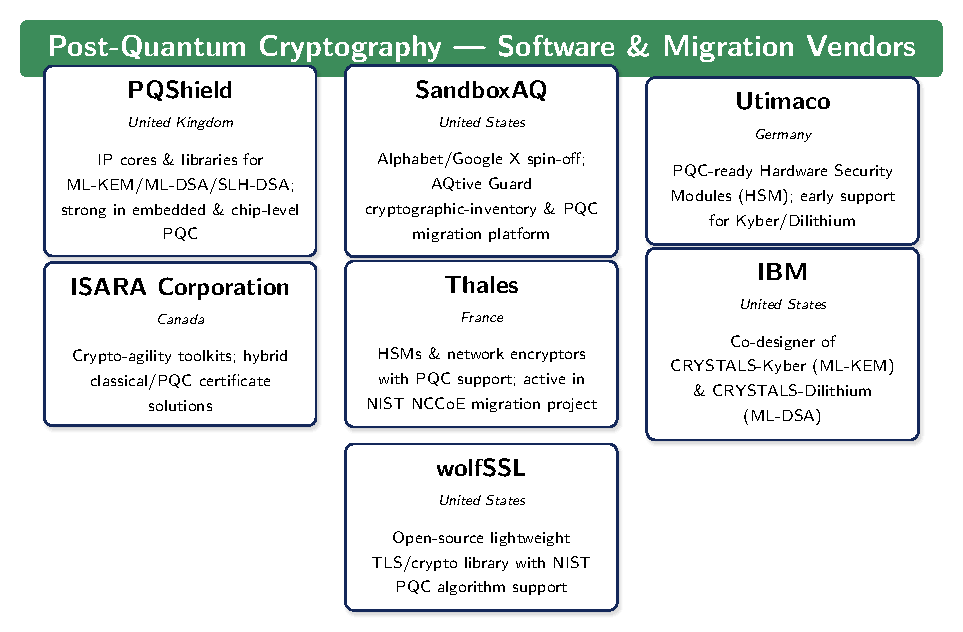
\includegraphics[width=0.98\linewidth]{figs/fig_pqc_vendors.pdf}
% TODO: لوگو -- نام‌های پیشنهادی فایل در figs/logos/README.txt
% \vspace{4pt}
% \includegraphics[height=1.1cm]{figs/logos/pqshield.png}\hfill
% \includegraphics[height=1.1cm]{figs/logos/sandboxaq.png}\hfill
% \includegraphics[height=1.1cm]{figs/logos/ibm.png}
\caption{شرکت‌های فعال در توسعهٔ نرم‌افزار و سخت‌افزار رمزنگاری پساکوانتومی \Cite{tqi2026pqccompanies,pqshield2026,nccoe2024migration}}
\label{fig:pqcvendors}
\end{figure}

شایان ذکر است که دو الگوریتم اصلی استانداردشدهٔ \lr{NIST} -- یعنی \lr{ML-KEM} و \lr{ML-DSA} -- به‌ترتیب از طرح‌های \lr{CRYSTALS-Kyber} و \lr{CRYSTALS-Dilithium} مشتق شده‌اند که با مشارکت مستقیم پژوهشگران \lr{IBM} طراحی شده بودند؛ این نکته نشان می‌دهد که مرز میان «استاندارد دولتی» و «محصول صنعتی» در حوزهٔ \lr{PQC} بسیار کم‌رنگ است و بومی‌سازی این فناوری می‌تواند از همان کتابخانه‌های متن‌باز (مانند \lr{liboqs} یا \lr{wolfSSL}) آغاز شود.

%=====================================================================

\chapter{مبانی نظری توزیع کلید کوانتومی}
%=====================================================================

\section{اصول فیزیکی زیربنایی}

امنیت \lr{QKD} بر خلاف رمزنگاری کلاسیک، متکی به دشواری محاسباتی یک مسئلهٔ ریاضی نیست، بلکه مستقیماً از قوانین بنیادین مکانیک کوانتومی نتیجه می‌شود. دو اصل کلیدی در این میان نقش تعیین‌کننده دارند:

\begin{definition}[اصل عدم‌قطعیت در اندازه‌گیری]
اندازه‌گیری یک حالت کوانتومی ناشناخته در یک پایهٔ اندازه‌گیری دلخواه، به‌طور کلی آن حالت را برهم می‌زند؛ مگر آنکه پایهٔ اندازه‌گیری با پایه‌ای که حالت در آن تهیه شده، منطبق باشد.
\end{definition}

\begin{theorem}[قضیهٔ عدم-شبیه‌سازی \lr{\cite{wootters1982}}]
هیچ عملگر یکانی (فیزیکی) وجود ندارد که بتواند یک حالت کوانتومی دلخواه و ناشناخته $\lvert\psi\rangle$ را بدون تغییر در حالت اصلی، به‌طور کامل روی یک سامانهٔ کمکی کپی کند.
\end{theorem}

نتیجهٔ مستقیم این قضیه برای امنیت ارتباطات آن است که یک شنودگر \lr{(Eve)} \textbf{اصولاً نمی‌تواند} فوتون‌های حامل کلید را رهگیری، کپی و بدون تغییر ارسال کند؛ هرگونه تلاش برای اندازه‌گیری یا کپی‌برداری از حالت کوانتومی، اختلال آماری قابل‌کشفی در نرخ خطای بیت کوانتومی (تعریف در بخش \lr{2.3}) ایجاد می‌کند. این ویژگی -- که در رمزنگاری کلاسیک هیچ مابه‌ازایی ندارد -- پایهٔ \textbf{امنیت اثبات‌پذیر اطلاعاتی} \lr{(Information-Theoretic Security)} در \lr{QKD} است.

\section{پروتکل \lr{BB84}}

نخستین و پرکاربردترین پروتکل \lr{QKD}، پروتکل \lr{BB84}\LTRfootnote{Named after its inventors, Bennett and Brassard, and the publication year 1984.} است که در سال $1984$ توسط بنت و براسارد\LTRfootnote{Charles H. Bennett and Gilles Brassard} \lr{\cite{bennett1984}} پیشنهاد شد. شکل \ref{fig:bb84} گردش کار کلی این پروتکل را نشان می‌دهد.

\begin{figure}[htbp]
\centering
\begin{tikzpicture}[
  node distance=1.2cm,
  box/.style={rectangle,draw,thick,rounded corners,minimum width=2.6cm,minimum height=1cm,align=center,fill=blue!8},
]
\node[box] (alice) {\lr{Alice}\\(فرستنده)};
\node[box,right=6.3cm of alice] (bob) {\lr{Bob}\\(گیرنده)};
\draw[-{Stealth[length=3mm]},thick,blue!60!black] (alice) -- node[above,font=\footnotesize]{\rl{کانال کوانتومی (فوتون‌های تکی)}} (bob);
\draw[-{Stealth[length=3mm]},thick,red!60!black] ($(alice.south)+(0,-0.4)$) -- node[below,font=\footnotesize]{کانال کلاسیک (تطبیق پایه، تصحیح خطا، تقطیر محرمانگی)} ($(bob.south)+(0,-0.4)$);
\node[below=1.1cm of alice, align=right, font=\footnotesize] (a2) {\lr{1.} تولید بیت‌های تصادفی\\\lr{2.} انتخاب تصادفی پایه ($+/\times$)\\\lr{3.} کدگذاری و ارسال قوبیت‌ها};
\node[below=1.1cm of bob, align=right, font=\footnotesize] (b2) {\lr{1.} انتخاب تصادفی پایهٔ اندازه‌گیری\\\lr{2.} اندازه‌گیری قوبیت‌ها\\\lr{3.} غربال‌سازی کلید \lr{(Key Sifting)}};
\end{tikzpicture}
\caption{شمای کلی پروتکل \lr{BB84}: تبادل کلید کوانتومی بین \lr{Alice} و \lr{Bob}}
\label{fig:bb84}
\end{figure}

برای نمایش دقیق‌تر ترتیب زمانی پیام‌ها میان دو طرف، شکل \ref{fig:bb84seq} همان پروتکل را در قالب نمودار توالی \lr{(Sequence Diagram)} نشان می‌دهد که هفت گام اصلی توضیح داده‌شده در ادامه را به‌ترتیب دربر می‌گیرد.

\begin{figure}[htbp]
\centering
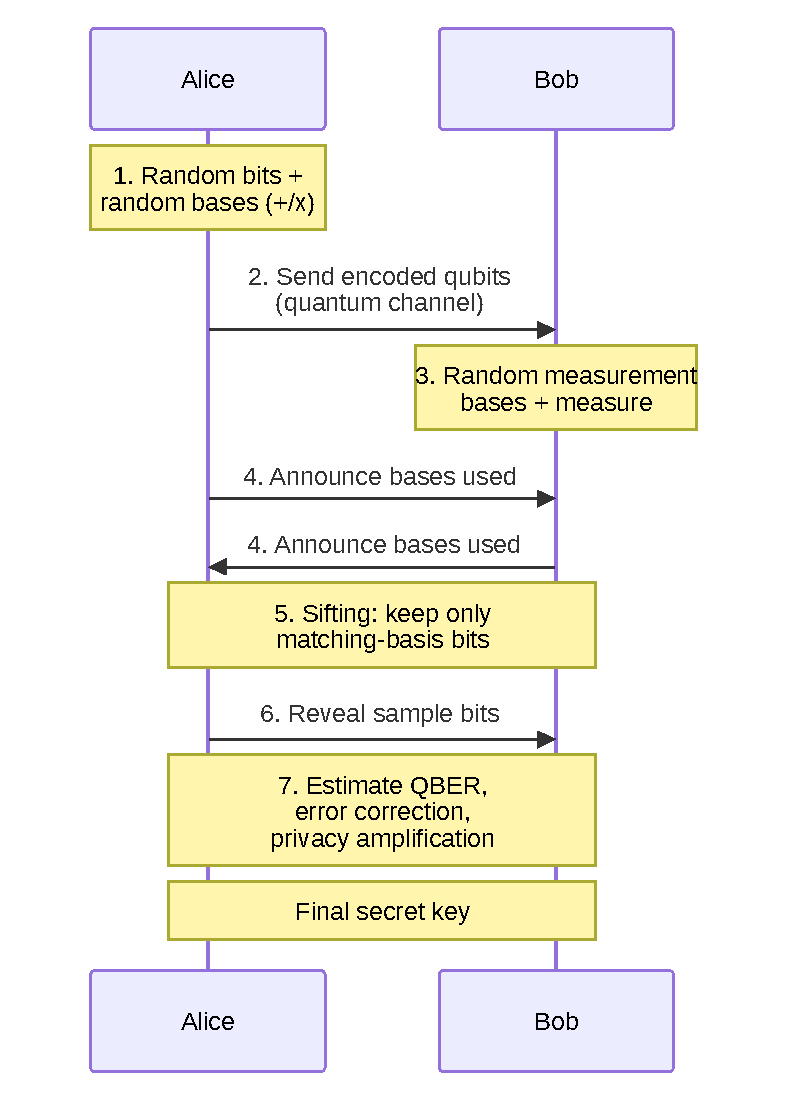
\includegraphics[width=0.75\linewidth]{figs/fig_bb84_sequence.pdf}
\caption{نمودار توالی زمانی پروتکل \lr{BB84} از تولید بیت تصادفی تا استخراج کلید نهایی}
\label{fig:bb84seq}
\end{figure}

مراحل اصلی پروتکل \lr{BB84} به شرح زیر است:

\begin{enumerate}
\item \textbf{تهیهٔ حالت \lr{(State Preparation)}:} \lr{Alice} برای هر بیت کلید، به‌صورت تصادفی یکی از دو پایهٔ متعامد -- پایهٔ مستطیلی ($+$) یا پایهٔ قطری ($\times$) -- را انتخاب کرده و بیت را روی حالت قطبش فوتون کدگذاری می‌کند.
\item \textbf{انتقال:} فوتون‌ها از طریق کانال کوانتومی (معمولاً فیبر نوری تاریک \lr{(Dark Fiber)} در طول‌موج $1550$ نانومتر یا کانال فضای آزاد/ماهواره‌ای) به \lr{Bob} ارسال می‌شوند.
\item \textbf{اندازه‌گیری:} \lr{Bob} برای هر فوتون دریافتی، به‌طور مستقل و تصادفی یکی از دو پایه را برای اندازه‌گیری انتخاب می‌کند.
\item \textbf{تطبیق پایه \lr{(Basis Reconciliation)}:} \lr{Alice} و \lr{Bob} از طریق یک کانال کلاسیک \textbf{احراز‌هویت‌شده} (نه لزوماً محرمانه)، پایه‌های انتخابی خود را -- بدون افشای مقدار بیت‌ها -- مقایسه کرده و تنها بیت‌هایی را نگه می‌دارند که در آن‌ها پایهٔ فرستنده و گیرنده یکسان بوده است. این مرحله «کلید غربال‌شده» \lr{(Sifted Key)} را تولید می‌کند.
\item \textbf{برآورد نرخ خطا و تصحیح خطا:} با مقایسهٔ زیرمجموعه‌ای تصادفی از کلید غربال‌شده، نرخ خطای بیت کوانتومی برآورد می‌شود.
\item \textbf{تقطیر محرمانگی \lr{(Privacy Amplification)}:} با استفاده از توابع درهم‌سازی جهانی \lr{(Universal Hashing)}، طول کلید کاهش داده می‌شود تا هرگونه اطلاعات نشت‌یافته به شنودگر عملاً به صفر برسد و «کلید نهایی امن» تولید شود.
\end{enumerate}

\section{نرخ خطای بیت کوانتومی و نرخ کلید امن}

نرخ خطای بیت کوانتومی \lr{(Quantum Bit Error Rate -- QBER)} مهم‌ترین شاخص کیفیت و امنیت یک پیوند \lr{QKD} است و به‌صورت زیر تعریف می‌شود:

\begin{equation}
\label{eq:qber}
\mathrm{QBER} = \frac{N_{\text{error}}}{N_{\text{total}}}
\end{equation}

که در آن $N_{\text{error}}$ تعداد بیت‌های نادرست در نمونهٔ آزمایش‌شده و $N_{\text{total}}$ تعداد کل بیت‌های غربال‌شدهٔ نمونه‌برداری‌شده است. در عمل، یک آستانهٔ امنیتی مشخص (برای \lr{BB84} معمولاً در حدود $11\%$) وجود دارد که فراتر از آن، امکان استخراج کلید امن از نظر تئوری اطلاعات وجود ندارد و ارتباط باید قطع شود.

با در نظر گرفتن اثرات عملی نظیر تلفات کانال، نویز آشکارساز و حملات نشت‌اطلاعات از کانال جانبی، نرخ کلید امن نهایی $R$ با فرمول تعمیم‌یافتهٔ \lr{GLLP}\LTRfootnote{Gottesman, Lo, Lütkenhaus, and Preskill} \lr{\cite{gllp2004}} به‌صورت زیر تخمین زده می‌شود:

\begin{align}
\label{eq:gllp}
R \;\geq\; q \Big\{ -Q_{\mu}\, f(E_{\mu})\, H_2(E_{\mu}) \;+\; Q_1 \big[1 - H_2(e_1)\big] \Big\}
\end{align}

که در آن $q$ کارایی پروتکل (برای \lr{BB84} با غربال‌سازی معمولی $q=1/2$)، $Q_{\mu}$ نرخ شمارش کلی، $E_{\mu}$ نرخ خطای کلی، $f(E_{\mu})$ کارایی الگوریتم تصحیح خطا (معمولاً بین $1.1$ تا $1.2$)، $Q_1$ و $e_1$ به‌ترتیب نرخ شمارش و نرخ خطای رویدادهای تک‌فوتونی، و $H_2(\cdot)$ تابع آنتروپی دودویی شانون است:

\begin{equation}
H_2(x) = -x\log_2(x) - (1-x)\log_2(1-x)
\end{equation}

این رابطه نشان می‌دهد که نرخ کلید امن با افزایش فاصلهٔ انتقال (و درنتیجه افزایش تلفات و کاهش $Q_1$) به‌صورت نمایی افت می‌کند -- محدودیتی بنیادین که در فصل بعد، معماری‌های عملی برای غلبه بر آن معرفی می‌شوند.

%=====================================================================

\include{chapters/03-qkd-architecture}
\include{chapters/05-hybrid-qkd-pqc}
\include{chapters/06-banking-applications}
\include{chapters/07-global-experience}
\chapter{طرح پیشنهادی برای پیاده‌سازی در تهران}
%=====================================================================

\section{اصول طراحی}

با توجه به تجربهٔ بین‌المللی مرورشده در فصل قبل، طرح پیشنهادی برای تهران بر اصول زیر استوار است:

\begin{itemize}
\item \textbf{شروع کلان‌شهری، نه ملی:} به‌جای یک کریدور بین‌شهری پرهزینه، فاز نخست بر یک حلقهٔ \lr{QKD} کلان‌شهری با شعاع کمتر از $50$ کیلومتر متمرکز است -- مشابه رویکرد پایلوت‌های موفق \lr{HSBC} در لندن و \lr{JPMorgan} در نیویورک/نیوجرسی؛
\item \textbf{اولویت با گره‌های با بیشترین ارزش دارایی اطلاعاتی:} بانک مرکزی، مراکز دادهٔ بانک‌های بزرگ دولتی و خصوصی، و مراکز حساس دولتی؛
\item \textbf{توپولوژی حلقه‌ای \lr{(Ring)}} برای تاب‌آوری در برابر قطعی یک بخش از فیبر؛
\item \textbf{معماری ترکیبی از ابتدا:} پیاده‌سازی هم‌زمان لایهٔ \lr{PQC (ML-KEM/ML-DSA)} در نرم‌افزار، به‌موازات ساخت زیرساخت فیزیکی \lr{QKD}، تا از همان فاز نخست پوشش امنیتی فراهم باشد؛
\item \textbf{استفاده از فیبر تاریک موجود شرکت مخابرات ایران} در حد امکان، برای کاهش هزینهٔ حفاری و کابل‌کشی جدید.
\end{itemize}

\section{توپولوژی پیشنهادی}

شکل \ref{fig:tehran} توپولوژی حلقه‌ای پیشنهادی را نشان می‌دهد. شش گرهٔ اصلی (نمادین و برای اهداف نمایش فنی) در نظر گرفته شده‌اند:

\begin{enumerate}
\item \textbf{بانک مرکزی جمهوری اسلامی ایران} -- به‌عنوان گرهٔ ریشهٔ اعتماد \lr{(Root of Trust)} و مرکز مدیریت کلید سراسری؛
\item \textbf{مرکز دادهٔ اصلی شبکهٔ بانکی (شتاب/شاپرک)} -- برای ایمن‌سازی زیرساخت تسویهٔ بین‌بانکی؛
\item \textbf{مرکز دادهٔ پشتیبان بانکی} -- جهت تداوم کسب‌وکار و مسیر جایگزین؛
\item \textbf{شرکت ارتباطات زیرساخت / مخابرات ایران} -- به‌عنوان مالک و بهره‌بردار فیبر تاریک؛
\item \textbf{مرکز دادهٔ دولتی حساس (مطابق سیاست ملی فضای مجازی)}؛
\item \textbf{مرکز پژوهشی/دانشگاهی} (برای انتقال دانش فنی و پایش مستمر امنیت پروتکل).
\end{enumerate}

\begin{figure}[htbp]
\centering
\begin{tikzpicture}[
  nd/.style={rectangle,draw,thick,rounded corners,minimum width=3cm,minimum height=1.1cm,align=center,fill=green!10,font=\scriptsize},
  link/.style={thick,blue!50!black}
]
\def\R{3.6}
\def\N{6}
\node[nd,fill=goldacc!25] (r0) at (90:\R) {بانک مرکزی\\(ریشهٔ اعتماد)};
\node[nd] (r1) at (30:\R) {مرکز دادهٔ\\شتاب/شاپرک};
\node[nd] (r2) at (-30:\R) {مرکز دادهٔ\\پشتیبان بانکی};
\node[nd] (r3) at (-90:\R) {مخابرات ایران\\(هاب فیبر)};
\node[nd] (r4) at (-150:\R) {مرکز دادهٔ\\دولتی حساس};
\node[nd] (r5) at (150:\R) {مرکز\\پژوهشی/دانشگاهی};
\foreach \a/\b in {r0/r1,r1/r2,r2/r3,r3/r4,r4/r5,r5/r0}{
  \draw[link] (\a) -- (\b);
}
\node[align=center,font=\tiny] at (0,0) {توپولوژی حلقه‌ای\\(تاب‌آور در برابر\\قطعی تک‌نقطه‌ای)};
\end{tikzpicture}
\caption{توپولوژی پیشنهادی حلقهٔ \lr{QKD} کلان‌شهری تهران (فاز نخست، نمادین)}
\label{fig:tehran}
\end{figure}

\textbf{تذکر مهم:} فاصلهٔ واقعی و مکان دقیق هر یک از این نهادها باید در فاز مطالعهٔ امکان‌سنجی (فصل \lr{12}، فاز \lr{1}) با همکاری شرکت مخابرات ایران و اپراتورهای دارای مجوز فیبر تاریک، به‌طور دقیق نقشه‌برداری و تلفات واقعی فیبر اندازه‌گیری شود. با توجه به وسعت جغرافیایی تهران بزرگ، محتمل است حداقل یک گرهٔ مورد اعتماد میانی (مطابق بخش \lr{3.2}) برای اتصال گره‌های دورتر (مثلاً مراکز داده در جنوب یا غرب تهران) لازم باشد.

\section{فناوری‌های پیشنهادی برای هر لایه}

جدول \ref{tab:techstack} پشتهٔ فناوری پیشنهادی برای هر لایهٔ معماری را ارائه می‌دهد.

\begin{table}[htbp]
\centering
\caption{پشتهٔ فناوری پیشنهادی برای طرح تهران}
\label{tab:techstack}
\small
\begin{tabular}{p{3cm}p{5.8cm}p{5.5cm}}
\toprule
\textbf{لایه} & \textbf{فناوری/پروتکل پیشنهادی} & \textbf{دلیل انتخاب} \\
\midrule
لایهٔ فیزیکی \lr{QKD} & \lr{DV-QKD} مبتنی بر \lr{decoy-state BB84} با گزینهٔ ارتقا به \lr{MDI-QKD} برای گره‌های حساس & بالاترین بلوغ تجاری و بیشترین تعداد تولیدکنندهٔ معتبر (جدول \ref{tab:protocols}) \\
کانال انتقال & فیبر تک‌مود اختصاصی (تاریک) در باند \lr{O} یا \lr{C}؛ در صورت کمبود فیبر، سامانهٔ \lr{Multiplexed QKD} برای هم‌زیستی با ترافیک کلاسیک & کاهش هزینهٔ زیرساخت با اجتناب از حفاری مضاعف \Cite{toshiba2026qkd} \\
مدیریت کلید & \lr{KMS} سازگار با \lr{ETSI GS QKD 014} & سازگاری چندفروشنده‌ای و امکان ارتقای آتی \\
لایهٔ نرم‌افزاری \lr{PQC} & \lr{ML-KEM-768} برای تبادل کلید، \lr{ML-DSA-65} برای امضای تراکنش‌ها & تعادل مناسب امنیت/کارایی برای بار تراکنشی بانکی سنگین \\
رمزگذار خط \lr{(Line Encryptor)} & رمزگذار سازگار با \lr{QKD} در لایهٔ $1$/$2$ با پشتیبانی \lr{AES-256}\LTRfootnote{Advanced Encryption Standard, 256-bit key} & استاندارد صنعتی پذیرفته‌شده در پروژه‌های \lr{HSBC} و \lr{JPMorgan} \\
\bottomrule
\end{tabular}
\end{table}

%=====================================================================

\chapter{تجهیزات پیشنهادی و برآورد هزینه}
\label{chap:cost}
%=====================================================================

\section{مأخذ برآورد}

برآوردهای این فصل بر مبنای قیمت‌های عمومی منتشرشده توسط تولیدکنندگان و گزارش‌های تحلیل بازار جهانی است و \textbf{صرفاً برای برنامه‌ریزی اولیهٔ بودجه} ارائه می‌شود؛ قیمت نهایی باید از طریق استعلام رسمی و مناقصهٔ بین‌المللی/داخلی مطابق مقررات ساماندهی خرید کالای دولتی مشخص شود. لازم به ذکر است که به‌دلیل تحریم‌های فناوری، ممکن است دسترسی مستقیم به برخی تولیدکنندگان غربی (\lr{ID Quantique}، \lr{Toshiba}) با محدودیت مواجه باشد و لازم است گزینه‌های جایگزین (تأمین از طریق کشورهای ثالث، یا توسعهٔ داخلی نمونهٔ اولیه با همکاری مراکز پژوهشی داخلی) نیز به‌موازات ارزیابی شود.

\section{هزینهٔ تجهیزات هر گره}

بر اساس داده‌های صنعتی، هزینهٔ یک زوج سامانهٔ \lr{QKD} تجاری (فرستنده و گیرنده) بسته به نسل فناوری و نرخ کلید، در بازهٔ وسیعی قرار می‌گیرد: نمونه‌های اولیهٔ تجاری در حدود $82000$ دلار برای یک زوج \Cite{mittech2009}، سامانه‌های میان‌رده در بازهٔ $150000$ تا $400000$ دلار \Cite{arxiv0905report}، و آشکارسازهای فوق‌پیشرفتهٔ نانوسیم ابررسانا برای برد بلند در حدود $100000$ یورو برای هر واحد \Cite{techtimes2026sweden}. برای یک شبکهٔ متروپلیتن سازمانی متوسط با دو تا سه سایت در شعاع $50$ کیلومتری، هزینهٔ کل معمولاً بین $500000$ تا $3$ میلیون دلار برآورد می‌شود \Cite{marketintelo2026}.

\begin{table}[htbp]
\centering
\caption{برآورد هزینهٔ اجزای اصلی طرح پایلوت تهران (شش گره، توپولوژی حلقه‌ای)}
\label{tab:cost}
\small
\begin{tabular}{p{5.5cm}p{3.5cm}p{4.5cm}}
\toprule
\textbf{قلم هزینه} & \textbf{برآورد (میلیون دلار)} & \textbf{توضیح} \\
\midrule
سامانه‌های \lr{QKD} (شش زوج فرستنده/گیرنده) & $1.8$ -- $3.2$ & بر مبنای سامانهٔ میان‌رده تا پیشرفته \Cite{idq2025cerberis,toshiba2026qkd} \\
\lr{KMS} و نرم‌افزار مدیریت کلید & $0.3$ -- $0.5$ & شامل مجوز نرم‌افزار و یکپارچه‌سازی \lr{API} \\
فیبر تاریک (اجاره/حفاری تکمیلی) & $0.5$ -- $0.9$ & بسته به میزان فیبر موجود مخابرات ایران \\
رمزگذارهای خط و تجهیزات شبکه & $0.4$ -- $0.8$ & رمزگذار \lr{AES-256} سازگار با \lr{QKD} \\
یکپارچه‌سازی \lr{PQC} در نرم‌افزار بانکی & $0.3$ -- $0.6$ & پیاده‌سازی \lr{ML-KEM/ML-DSA} در زیرساخت پیام‌رسانی بانکی \\
آموزش، ممیزی امنیتی و گواهی‌دهی & $0.2$ -- $0.4$ & شامل آزمون نفوذ و ارزیابی مستقل \\
بهره‌برداری و نگهداشت سالانه (سال اول) & $0.3$ -- $0.5$ & پشتیبانی فنی، پایش و به‌روزرسانی \\
\midrule
\textbf{جمع کل برآوردی (فاز پایلوت)} & \textbf{$3.8$ -- $6.9$} & \\
\bottomrule
\end{tabular}
\end{table}

شکل \ref{fig:costchart} توزیع تقریبی این هزینه‌ها را برای سناریوی میانی نشان می‌دهد.

\begin{figure}[htbp]
\centering
\begin{tikzpicture}
\begin{axis}[
  ybar,
  bar width=16pt,
  width=12.5cm,height=6.5cm,
  symbolic x coords={تجهیزات \lr{QKD},\lr{KMS},فیبر,رمزگذار,\lr{PQC},آموزش,بهره‌برداری},
  xtick=data,
  x tick label style={font=\scriptsize,rotate=20,anchor=east},
  ylabel={میلیون دلار},
  nodes near coords,
  nodes near coords style={font=\scriptsize},
  ymin=0,
  ymajorgrids=true,
  grid style=dashed,
]
\addplot[fill=blue!35] coordinates {
  (تجهیزات \lr{QKD},2.5) (\lr{KMS},0.4) (فیبر,0.7) (رمزگذار,0.6) (\lr{PQC},0.45) (آموزش,0.3) (بهره‌برداری,0.4)
};
\end{axis}
\end{tikzpicture}
\caption{توزیع تقریبی برآورد هزینهٔ فاز پایلوت (سناریوی میانی)}
\label{fig:costchart}
\end{figure}

برای مشاهدهٔ سریع‌تر سهم نسبی هر قلم هزینه از کل بودجه، شکل \ref{fig:costpie} همان داده‌ها را به‌صورت نمودار دایره‌ای نمایش می‌دهد؛ همان‌طور که مشخص است، تنها تجهیزات \lr{QKD} به‌تنهایی نزدیک به نیمی از کل بودجهٔ فاز پایلوت را تشکیل می‌دهد.

\begin{figure}[htbp]
\centering
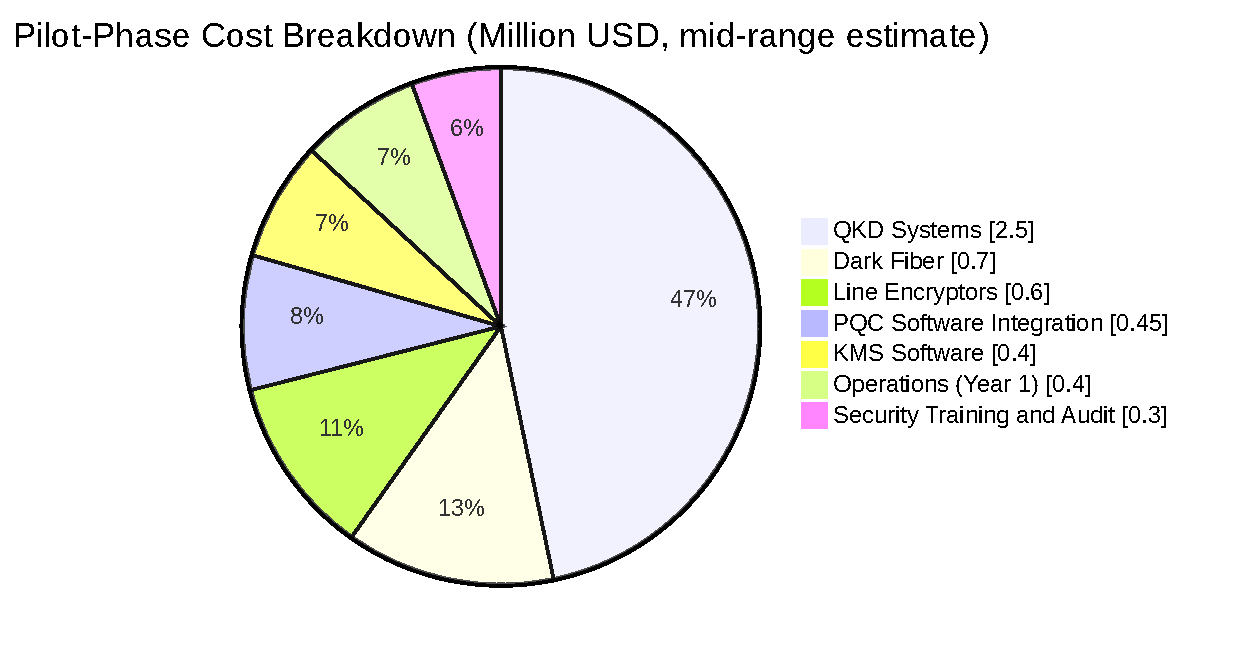
\includegraphics[width=0.72\linewidth]{figs/fig_cost_pie.pdf}
\caption{سهم نسبی هر قلم از برآورد هزینهٔ فاز پایلوت}
\label{fig:costpie}
\end{figure}

\section{هزینهٔ توسعهٔ آتی به مقیاس ملی}

بازار جهانی \lr{QKD} در افق سال $2035$ به حدود $20$ میلیارد دلار برآورد می‌شود \Cite{toshiba2020launch}. توسعهٔ طرح از مقیاس پایلوت کلان‌شهری به یک کریدور بین‌شهری (مثلاً تهران--اصفهان یا تهران--مشهد) نیازمند سرمایه‌گذاری در مقیاس ده‌ها میلیون دلار و افق زمانی چندساله خواهد بود و پیشنهاد می‌شود صرفاً پس از تکمیل موفق و ارزیابی امنیتی فاز پایلوت بررسی شود.

%=====================================================================

\include{chapters/10-security-risk}
\chapter{نقشهٔ راه اجرایی}
\label{ch:roadmap}
%=====================================================================

\section{منطق فازبندی}

نقشهٔ راهی که در این فصل ارائه می‌شود، بر یک اصل ساده بنا شده است: در پروژه‌ای که بخش قابل‌توجهی از تجهیزات حیاتی آن (بخش \ref{sec:labequipment}) به‌دلیل تحریم فناوری با عدم‌قطعیت زمان تحویل مواجه است، بزرگ‌ترین خطر برای زمان‌بندی، پیچیدگی مهندسی نیست بلکه \textbf{زنجیرهٔ تأمین} است. به همین دلیل، برخلاف الگوی متداول «ابتدا طراحی کامل شود، سپس خرید انجام گیرد، سپس ساخته شود»، در این طرح فاز تدارکات اقلام حساس از همان ماه‌های نخست و به‌موازات فازهای تحقیق و طراحی آغاز می‌شود. اگر این همپوشانی رعایت نشود، تیم پروژه می‌تواند در پایان ماه ششم طراحی کاملی در دست داشته باشد اما همچنان چند ماه دیگر منتظر رسیدن یک آشکارساز تک‌فوتون بماند -- سناریویی که کاملاً قابل‌پیش‌بینی و قابل‌اجتناب است.

فازبندی به نه بخش اصلی تقسیم شده که سه مورد از آن‌ها (فاز \lr{0}، فاز \lr{2} و فاز \lr{6}) به‌صورت موازی با بقیه پیش می‌روند نه به‌صورت متوالی؛ توضیح هر فاز، همراه با نتیجهٔ ملموسی که در پایان آن باید روی میز باشد، در ادامه آمده است.

\subsection*{فاز \texorpdfstring{\lr{0}}{۰} -- تحقیق و توسعه (ماه \texorpdfstring{\lr{1}}{۱} تا \texorpdfstring{\lr{3}}{۳})}
این فاز، پایهٔ فکری کل پروژه است و شامل مرور نظام‌مند ادبیات فنی روز (از جمله منابع فصل‌های \ref{chap:hybrid} و بخش \ref{sec:pqcfoundations})، انتخاب نهایی پروتکل \lr{QKD} (بین \lr{decoy-state BB84}، \lr{MDI-QKD} و \lr{TF-QKD}) متناسب با فاصلهٔ واقعی گره‌های تهران، انتخاب مجموعهٔ الگوریتم‌های \lr{PQC} استاندارد \lr{NIST} (\lr{ML-KEM}، \lr{ML-DSA}، \lr{SLH-DSA} به‌عنوان پشتیبان)، و شبیه‌سازی نرم‌افزاری کامل کانال و پروتکل پیش از هرگونه ساخت سخت‌افزاری است. خروجی این فاز یک سند فنی مرجع است که مبنای تصمیم‌گیری تمام فازهای بعدی قرار می‌گیرد.

\subsection*{فاز \texorpdfstring{\lr{1}}{۱} -- طراحی شبکه (ماه \texorpdfstring{\lr{2}}{۲} تا \texorpdfstring{\lr{4}}{۴})}
موازی با پایان‌یافتن فاز \lr{0}، تیم شبکه باید نقشه‌برداری فیبر تاریک موجود مخابرات را انجام دهد، تلفات واقعی مسیرهای پیشنهادی را با اندازه‌گیری میدانی (نه صرفاً برآورد نظری) تعیین کند، گره‌های نهایی را قطعی و توپولوژی حلقه‌ای شش‌گانه را نهایی نماید، و سند الزامات امنیت فیزیکی سایت‌ها را تدوین کند.

\subsection*{فاز \texorpdfstring{\lr{2}}{۲} -- تدارکات و تأمین تجهیزات (ماه \texorpdfstring{\lr{2}}{۲} تا \texorpdfstring{\lr{8}}{۸}، موازی)}
مهم‌ترین فاز از منظر مدیریت ریسک. سفارش اقلام کم‌ریسک (سرور، شبکه، برد \lr{FPGA} میان‌رده) می‌تواند در همان هفته‌های نخست و با زمان تحویل کوتاه انجام شود؛ اما سفارش اقلام پرریسک تحریمی -- آشکارساز تک‌فوتون، مدولاتور نوری، \lr{QRNG} سخت‌افزاری (بخش \ref{sec:labequipment}) -- باید همزمان و بدون تأخیر آغاز شود، چون این دقیقاً همان اقلامی هستند که زمان تحویل چندماهه و غیرقطعی دارند. توصیهٔ صریح این نقشهٔ راه آن است که مسیر تأمین این اقلام حساس، به‌موازات مسیر توسعهٔ داخلی جایگزین (همکاری با مراکز پژوهشی اپتوالکترونیک داخلی) دنبال شود تا در صورت تأخیر یا شکست یک مسیر، پروژه به‌طور کامل متوقف نشود.

\subsection*{فاز \texorpdfstring{\lr{3}}{۳} -- نمونهٔ اولیهٔ آزمایشگاهی \texorpdfstring{\lr{QKD}}{QKD} (ماه \texorpdfstring{\lr{4}}{۴} تا \texorpdfstring{\lr{8}}{۸})}
با رسیدن نخستین محمولهٔ تجهیزات، سامانهٔ فرستنده/گیرنده روی میز آزمایشگاه (نه در فیبر میدانی) مونتاژ و کالیبره می‌شود: هم‌ترازی نوری، کالیبراسیون آشکارساز، و اندازه‌گیری نرخ خطای بیت کوانتومی (\lr{QBER}) در یک حلقهٔ فیبر کوتاه و کاملاً کنترل‌شده. این فاز عمداً پیش از هرگونه استقرار میدانی قرار گرفته تا خطاهای اساسی طراحی، پیش از صرف هزینهٔ حفاری و نصب فیبر شهری کشف شوند.

\subsection*{فاز \texorpdfstring{\lr{4}}{۴} -- پیوند آزمایشی میدانی دوگانه (ماه \texorpdfstring{\lr{7}}{۷} تا \texorpdfstring{\lr{10}}{۱۰})}
انتقال سامانهٔ اثبات‌شده از آزمایشگاه به نخستین پیوند واقعی میان دو گرهٔ اولویت‌دار (مثلاً بانک مرکزی و مرکز دادهٔ شتاب/شاپرک)، به‌عنوان اثبات مفهوم روی زیرساخت واقعی مخابراتی تهران.

\subsection*{فاز \texorpdfstring{\lr{5}}{۵} -- تکمیل حلقهٔ کلان‌شهری (ماه \texorpdfstring{\lr{9}}{۹} تا \texorpdfstring{\lr{13}}{۱۳})}
افزودن تدریجی باقی گره‌ها و تکمیل توپولوژی حلقه‌ای شش‌گانه، به‌همراه آزمون تاب‌آوری شبکه در برابر قطعی یک پیوند منفرد.

\subsection*{فاز \texorpdfstring{\lr{6}}{۶} -- لایهٔ نرم‌افزاری \texorpdfstring{\lr{PQC}}{PQC} (ماه \texorpdfstring{\lr{2}}{۲} تا \texorpdfstring{\lr{9}}{۹}، موازی)}
از بزرگ‌ترین مزیت‌های این طرح آن است که یکپارچه‌سازی \lr{ML-KEM/ML-DSA} در نرم‌افزار بانکی، کاملاً مستقل از سخت‌افزار فیزیکی \lr{QKD} پیش می‌رود و به هیچ‌یک از تأخیرهای احتمالی فازهای \lr{2} تا \lr{5} وابسته نیست. این استقلال به‌معنای آن است که حتی اگر تأمین سخت‌افزار کوانتومی با تأخیر مواجه شود، ارتقای امنیت رمزنگاری کلاسیک بانک همچنان طبق برنامه پیش می‌رود -- و از این جهت، فاز \lr{6} «شبکهٔ اطمینان» کل پروژه در برابر ریسک تحریم است.

\subsection*{فاز \texorpdfstring{\lr{7}}{۷} -- یکپارچه‌سازی کامل بانکی (ماه \texorpdfstring{\lr{10}}{۱۰} تا \texorpdfstring{\lr{14}}{۱۴})}
اتصال \lr{KMS} به سامانه‌های پیام‌رسانی مالی موجود و آزمون تراکنش‌های واقعی در محیط کنترل‌شده (\lr{sandbox})، پیش از هرگونه اتصال به محیط عملیاتی زندهٔ بانک.

\subsection*{فاز \texorpdfstring{\lr{8}}{۸} -- ممیزی امنیتی و بهره‌برداری پایدار (ماه \texorpdfstring{\lr{13}}{۱۳} تا \texorpdfstring{\lr{16}}{۱۶} و ادامه)}
انتقال به بهره‌برداری کامل، عبور از یک دور آزمون نفوذ مستقل، و آغاز برنامه‌ریزی برای توسعهٔ آتی به مقیاس بین‌شهری (بخش \ref{sec:pqcfoundations}، فصل \ref{chap:cost}).

\begin{figure}[htbp]
\centering
\begin{ganttchart}[
  hgrid,vgrid,
  bar/.append style={fill=blue!45},
  bar height=0.55,
  title height=1,
  x unit=0.62cm,
  y unit chart=0.62cm,
]{1}{16}
\gantttitle{بازهٔ زمانی (ماه)}{16} \\
\gantttitlelist{1,...,16}{1} \\
\ganttbar{فاز \lr{0}: تحقیق و توسعه}{1}{3} \\
\ganttbar{فاز \lr{1}: طراحی شبکه}{2}{4} \\
\ganttbar[bar/.append style={fill=red!45}]{فاز \lr{2}: تدارکات (پرریسک تحریمی)}{2}{8} \\
\ganttbar{فاز \lr{3}: نمونهٔ اولیهٔ آزمایشگاهی}{4}{8} \\
\ganttbar{فاز \lr{4}: پیوند آزمایشی میدانی}{7}{10} \\
\ganttbar{فاز \lr{5}: تکمیل حلقهٔ کلان‌شهری}{9}{13} \\
\ganttbar[bar/.append style={fill=green!45}]{فاز \lr{6}: لایهٔ نرم‌افزاری \lr{PQC}}{2}{9} \\
\ganttbar{فاز \lr{7}: یکپارچه‌سازی بانکی}{10}{14} \\
\ganttbar{فاز \lr{8}: ممیزی و بهره‌برداری}{13}{16}
\end{ganttchart}
\caption{نقشهٔ راه تفصیلی اجرای فاز پایلوت؛ نوار قرمز (فاز \lr{2}) گلوگاه اصلی ریسک تحریمی و نوار سبز (فاز \lr{6}) مسیر مستقل و کم‌ریسک \lr{PQC} نرم‌افزاری را نشان می‌دهد}
\label{fig:gantt}
\end{figure}

\section{دو سناریوی زمانی: دست‌بالا در برابر واقع‌بینانه}

از آنجا که مدت زمان فاز \lr{2} (تدارکات) بیش از هر عامل دیگری به شرایط بیرونی و غیرقابل‌کنترل تیم پروژه وابسته است، ارائهٔ یک عدد قطعی برای «طول کل پروژه» گمراه‌کننده خواهد بود. جدول \ref{tab:scenario} دو سناریوی صریح را در کنار هم می‌گذارد تا تصمیم‌گیرندگان بتوانند بودجه و انتظارات را بر مبنای واقعیت تنظیم کنند، نه بر مبنای خوش‌بینانه‌ترین حالت ممکن.

\begin{table}[htbp]
\centering
\caption{مقایسهٔ سناریوی دست‌بالا (خوش‌بینانه) و واقع‌بینانه برای افق زمانی طرح پایلوت}
\label{tab:scenario}
\small
\begin{tabular}{p{2.8cm}p{2.2cm}p{8.5cm}}
\toprule
\textbf{سناریو} & \textbf{افق کل} & \textbf{مفروضات کلیدی} \\
\midrule
دست‌بالا (خوش‌بینانه) & $12$ ماه & تأمین اقلام حساس تحریمی بدون تأخیر و در همان بازهٔ برنامه‌ریزی‌شده (ماه $2$ تا $6$) انجام شود؛ هیچ‌یک از گره‌های فیبر نیاز به حفاری تکمیلی نداشته باشند؛ تخصیص بودجه از همان ماه اول قطعی و بدون وقفهٔ اداری باشد. \\
واقع‌بینانه & $16$ تا $18$ ماه & فاز تدارکات اقلام حساس ($2$ تا $3$ قلم اصلی) با میانگین $3$ تا $5$ ماه تأخیر نسبت به برنامه مواجه شود؛ حداقل یک دور بازطراحی پس از آزمون آزمایشگاهی (فاز $3$) لازم باشد؛ فرآیندهای اداری تخصیص بودجه و مناقصهٔ دولتی $1$ تا $2$ ماه به زمان اولیه اضافه کنند. \\
\bottomrule
\end{tabular}
\end{table}

توصیهٔ این نقشهٔ راه آن است که در هرگونه سند رسمی ارائه‌شده به نهادهای تصمیم‌گیرنده، عدد \textbf{واقع‌بینانه} (نه دست‌بالا) به‌عنوان افق رسمی پروژه اعلام شود؛ اعلام عدد خوش‌بینانه به‌عنوان تعهد رسمی، رایج‌ترین علت شکست اعتبار پروژه‌های زیرساختی در برخورد اول با تأخیر اجتناب‌ناپذیر یک قلم تحریمی است.

\section{شاخص‌های کلیدی موفقیت \lr{(KPI)}}

\begin{itemize}
\item برقراری پایدار پیوند \lr{QKD} با نرخ خطای بیت کوانتومی کمتر از آستانهٔ امنیتی (رابطهٔ \ref{eq:qber}) به‌مدت حداقل $90$ روز متوالی؛
\item یکپارچه‌سازی موفق \lr{PQC (ML-KEM/ML-DSA)} در حداقل یک سامانهٔ پیام‌رسانی مالی داخلی؛
\item عبور موفق از یک دور آزمون نفوذ مستقل بدون یافتن آسیب‌پذیری بحرانی؛
\item تربیت حداقل $10$ متخصص داخلی در حوزهٔ طراحی، بهره‌برداری و ممیزی امنیت \lr{QKD/PQC}؛
\item دستیابی به حداقل یک منبع تأمین داخلی (حتی در سطح نمونهٔ اولیه) برای دست‌کم یکی از اقلام پرریسک تحریمی جدول \ref{tab:labgear}، به‌عنوان گام نخست کاهش وابستگی بلندمدت.
\end{itemize}

%=====================================================================

\chapter{جمع‌بندی و پیشنهادها}
%=====================================================================

فناوری توزیع کلید کوانتومی و رمزنگاری پساکوانتومی دیگر در مرحلهٔ آزمایشگاهی نیستند؛ همان‌طور که در فصل‌های \lr{6} و \lr{7} نشان داده شد، بانک‌های پیشرو جهان و کشورهایی نظیر چین، سوئد و سنگاپور، این فناوری‌ها را در محیط‌های عملیاتی واقعی به‌کار گرفته‌اند. با نهایی‌شدن استانداردهای \lr{NIST} در سال $2024$، مسیر مهاجرت به رمزنگاری پساکوانتومی از نظر فنی کاملاً روشن و قابل‌اجراست، و فناوری \lr{QKD} نیز -- به‌ویژه برای کاربردهای کلان‌شهری با فاصلهٔ کوتاه نظیر اتصال مراکز دادهٔ بانکی -- به بلوغ تجاری کافی رسیده است.

این پروپوزال پیشنهاد می‌کند که جمهوری اسلامی ایران، به‌عنوان گامی پیشدستانه در برابر تهدید «برداشت اکنون، رمزگشایی بعداً»، یک طرح پایلوت کلان‌شهری در تهران را با تمرکز بر اتصال بانک مرکزی و زیرساخت‌های تسویهٔ بانکی، هم‌زمان با آغاز فوری مهاجرت نرم‌افزاری به \lr{ML-KEM} و \lr{ML-DSA} در سطح کل شبکهٔ بانکی کشور، آغاز کند. اجرای موفق این طرح پایلوت -- با بودجهٔ برآوردی $3.8$ تا $6.9$ میلیون دلار و افق زمانی $12$ ماهه -- می‌تواند بستری برای توسعهٔ دانش فنی بومی، کاهش وابستگی راهبردی به فناوری خارجی، و ارتقای جایگاه ایران در حوزهٔ نوظهور امنیت کوانتومی منطقه فراهم آورد.

\textbf{پیشنهاد نهایی جهت اقدام:} تشکیل یک کارگروه مشترک میان بانک مرکزی، معاونت علمی، فناوری و اقتصاد دانش‌بنیان ریاست‌جمهوری، مرکز افتا، و شرکت مخابرات ایران برای آغاز فاز \lr{1} (امکان‌سنجی) ظرف مدت $60$ روز از تصویب این طرح.



\bibliographystyle{plainnat}
\bibliography{refs}

\end{document}
